\documentclass[aps,tightenlines,16pt]{ctexart}


\usepackage{amsmath,amsfonts,amssymb}
\usepackage{bbm} %空心字母数字
\usepackage{ctex}
\usepackage{float}
%\usepackage[dvips]{graphicx}
\usepackage[english]{babel}
\allowdisplaybreaks[4]  %公式环境换行
\numberwithin{equation}{section}
\usepackage{slashed} %费曼slashed
\usepackage[left=2cm,right=2cm,top=2.54cm,bottom=2.54cm]{geometry}
%\usepackage[dvipdfm,pdfstartview=FitH]{hyperref}
%\usepackage{cancel}
%\usepackage{forest}
%\usepackage{leftidx}  %设置上下标
\usepackage{cite}
\usepackage[justification=centering]{caption}
\usepackage{graphicx, subfigure}
\usepackage{indentfirst}  %段落首行缩进
\usepackage{hyperref}  %设定引用公式跳转链接
\usepackage{color}  %设置字体颜色
\usepackage{tikz,pgf}
%\usepackage{tikz-feynman} 
%\tikzfeynmanset{compat=1.1.0}
\usepackage{braket}
%\usepackage{txfonts}  %平行符号
%\usepackage{fancyhdr}  %左偶右奇
\usepackage{multirow}
\usepackage{booktabs}
\usepackage{cancel}   
\usepackage{threeparttable}  
\usepackage{diagbox}
\usepackage{extpfeil}  %等号上加文字
\usepackage{extarrows}

\usetikzlibrary{calc}
%\usetikzlibrary{arrows.meta}
\usetikzlibrary{intersections}
\usetikzlibrary{trees}
\usetikzlibrary{decorations.pathmorphing}
\usetikzlibrary{decorations.markings}
\usetikzlibrary{patterns}
\tikzset{
   global scale/.style={
      scale=#1,
      every node/.append style={scale=#1}},
   photon/.style={decorate, decoration={snake}, draw=red},
   nucleon/.style={draw=black, postaction={decorate},
      decoration={markings,mark=at position .55 with{\arrow[draw=black]{>}}}},
   pion/.style={draw=blue, postaction={decorate},
      decoration={markings,mark=at position .55 with{\arrow[draw=blue]{}}}},
    }


\newcommand{\bl}{\boldsymbol{l}}
\newcommand{\bk}{\boldsymbol{k}}
\newcommand{\bp}{\boldsymbol{p}}
\newcommand{\bP}{\boldsymbol{P}}
\newcommand{\bq}{\boldsymbol{q}}
\newcommand{\bA}{\boldsymbol{A}}
\newcommand{\bM}{\boldsymbol{M}}
\newcommand{\bV}{\boldsymbol{V}}
\newcommand{\ba}{\boldsymbol{a}}
\newcommand{\bb}{\boldsymbol{b}}
\newcommand{\bx}{\boldsymbol{x}}
\newcommand{\bep}{\boldsymbol{\epsilon}}
\newcommand{\bsi}{\boldsymbol{\sigma}}
\newcommand{\bL}{\boldsymbol{L}}
\newcommand{\bJ}{\boldsymbol{J}}
\newcommand{\br}{\boldsymbol{r}}
\newcommand{\bs}{\boldsymbol{s}}
\newcommand{\bS}{\boldsymbol{S}}
\newcommand{\bi}{\boldsymbol{i}}
\newcommand{\bI}{\boldsymbol{I}}
\newcommand{\bB}{\boldsymbol{B}}  
\newcommand{\sP}{\slashed{P}} 
\newcommand{\spp}{\slashed{p}} 
\newcommand{\sk}{\slashed{k}} 
\newcommand{\sq}{\slashed{q}}
\newcommand{\sD}{\slashed{D}} 
\newcommand{\sA}{\slashed{A}}
\newcommand{\sep}{\slashed{\epsilon}} 
\newcommand{\spar}{\slashed{\partial}} 
\newcommand{\Pmu}{P^\mu} 
\newcommand{\pmu}{p^\mu} 
\newcommand{\kmu}{k^\mu} 
\newcommand{\qmu}{q^\mu}
\newcommand{\gmu}{\gamma^\mu}
\newcommand{\bpi}{\boldsymbol{\pi}}
\newcommand{\btau}{\boldsymbol{\tau}}
\newcommand{\brho}{\boldsymbol{\rho}}
\newcommand{\md}{\mathrm{d}}
\newcommand{\mB}{\mathbf{B}}
\newcommand{\mO}{\mathcal{O}}
\newcommand{\mL}{\mathcal{L}}
\allowdisplaybreaks


\begin{document}\large
     %\title{手征微扰场论阅读笔记} 
     \title{手征微扰场论}
     
\renewcommand{\today}{\number\year 年 \number\month 月 \number\day 日}
 \author{王旭}
 \maketitle
 %\newpage
 \setlength{\parindent}{2em}  %首行缩进两个中文字符
 \hypersetup{hypertex=true,
            colorlinks=true,
            linkcolor=blue,
            anchorcolor=blue,
            citecolor=blue}  %设定引用公式跳转链接
 \renewcommand\thesubsection{\arabic {subsection}}
 \renewcommand\contentsname{目录}
\tableofcontents
\newpage 

\section{有效量子力学}
该章主要参考\cite{kaplan2016lectures}。
当我们在描述低能理论时,我们不需要知道其在高能区的表现。代价就是需要引入大量参数,而这些参数只能由实验给出。在考察有效量子场论前,我们先看看有效量子力学。

由于在相对论量子力学中,粒子与粒子的相互作用是点点相互作用,因此我们希望通过$\delta$函数来模拟散射势。
\subsection{1D散射}
考虑量子力学中的一维散射问题,假设有一方势阱,其函数为
\begin{align}
   V(x)=
   \begin{cases}
      -\frac{\alpha^2}{2m\Delta}, & 0\leq x \leq \Delta \\
      0 ,& \mbox{其余情况}
   \end{cases}   
\end{align}
其中$m$为粒子质量,$\Delta$为势阱宽度,$\frac{\alpha^2}{2m\Delta^2}$为势阱深度。可以通过计算薛定谔方程得到反射系数$R$为
\begin{align}
   R=\Big[\frac{4\kappa^2 k^2 \mbox{csc}^2(\kappa \Delta)}{(k^2-\kappa^2)}+1\Big]^{-1}
\end{align}
其中
\begin{align}
   k=\sqrt{2mE},\   \kappa=\sqrt{k^2+\frac{\alpha^2}{\Delta^2}}
\end{align}
在低能时,我们可以按照$k$展开反射系数,
\begin{align}\label{1d_R}
   R= -\frac{4}{\alpha^2 \mbox{sin}^2\alpha}\Delta^2 k^2 + \mathcal{O}(\Delta^4 k^4)
\end{align}
可以看到当$k \to 0$时,$R \to 1$,称这种相互作用为相关相互作用。

\subsubsection{利用$\delta$函数来模仿方势阱}

考虑此时有一$\delta$势阱,
\begin{align}
   V(x)=-\frac{g}{2m\Delta}\delta(x)
\end{align}
此处引入$\Delta$来保证$g$是无量纲的。依旧通过薛定谔方程可以计算得出反射系数为,
\begin{align}
   R=\Big[1+\frac{4k^2\Delta^2}{g^2}\Big]^{-1}=1-\frac{4k^2\Delta^2}{g^2}+\mathcal{O}(k^4)
\end{align}
在低能情况下,与(\ref{1d_R})比较可得,
\begin{align}
   g=\alpha \mbox{sin}\alpha
\end{align}
称为“匹配条件”。

\subsection{3D散射}
首先,{\color{red}可以普遍证明},对于任意势场,$k\mbox{cot}\delta$可以展开为
\begin{align}\label{kcot}
   k\mbox{cot}\delta=-\frac{1}{a_0}+\frac{1}{2}r_0 k^2+\mathcal{O}(k^4)
\end{align}
考虑一$s$波的散射,势函数如下,
\begin{align}
   V=\begin{cases}
      -\frac{\alpha^2}{m\Delta^2},& r < \Delta \\
          0, & r > \Delta
   \end{cases}
\end{align}
其中$a$是散射长度,$r$是有效力程。
同样可以通过求解薛定谔方程得到$k\mbox{cot}\delta$的关系式,为
\begin{align}
      k\mbox{cot}\delta=\frac{k(k\mbox{sin}\kappa\Delta+\kappa\mbox{cot}k\Delta\mbox{cos}\kappa\Delta}{k\mbox{cot}k\Delta\mbox{sin}\kappa\Delta-\kappa\mbox{cos}\kappa\Delta}
\end{align}
将其按照$k^2$展开可得,
\begin{align}
   k\mbox{cot}\delta=\frac{1}{\Delta}\Big(\frac{\mbox{tan}\alpha}{\alpha}-1\Big)^{-1}+\mathcal{O}(k^2)
\end{align}
与(\ref{kcot})比较可得,
\begin{align}\label{3d_m}
   a=-\Delta\Big(\frac{\mbox{tan}\alpha}{\alpha}-1\Big)
\end{align}
其关系如图所示,
\begin{figure}[h]\centering
   \renewcommand{\figurename}{图}
   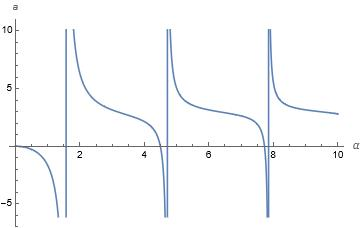
\includegraphics{3d_scattering.jpg}
\end{figure}

可以看到,势$\alpha$随散射长度$a$的变化,当$\alpha_c=(2n+1)\pi/2$时,$a$出现奇异性,对应着束缚态的出现。

\subsection{3D散射中的$\delta$函数}

我们首先给出3D散射下散射振幅
\begin{align}
   f=\frac{1}{k\mbox{cot}\delta-\mbox{i}k}
\end{align}
观察(\ref{3d_m}),由于$\alpha$是$\mO$(1),因此$a\sim\mO(\Delta)$,因此当势阱宽度趋于0时,散射振幅也趋于0,这种相互作用称为无关相互作用。因此无法用$\delta$函数来模拟球势阱。

如果我们用场$\psi$表示散射粒子,拉氏密度为
\begin{align}
   \mL = \psi^{\dagger}\Big(\mbox{i}\partial_t+\frac{\nabla^2}{2M}\Big)\psi-\frac{C_0}{4}\Big(\psi^{\dagger}\psi\Big)^2
\end{align}


\section{手征拉氏量}
该章主要参考\cite{scherer2011primer}





    
\newpage 

\renewcommand\refname{参考文献}

\bibliographystyle{unsrt}

\bibliography{ChPT}

\end{document}
